\section{8088 and 80188 (8-bit memory interface)}
Examples presented here pertain to the minimum mode. The microprocessor has 20 address pins, 8 data pins and 3 control signals containing $IO/\overline{M},~\overline{RD},~and~\overline{WR}$.
\subsection{Interfacing EPROM to the 8088}

\begin{figure}[h!]
  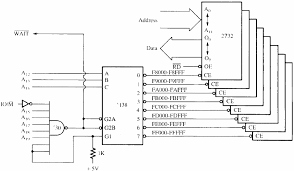
\includegraphics[width = 1\textwidth]{./figures/EPROM_2732.png}
  \caption{Interfacing EPROM 2732 to the 8088}
\end{figure}
\begin{itemize}
  \item EPROM 2732 has a memory access time of 450 ms. 8-8 aperates with 5 MHz clock allowing 460ns for the memory to access data. However, as decoders added time delay is 12ms, it is impossible for the memory to function with the 40ns delay. Therefore, generating a signal for inserting \textbf{WAIT} states is required.
  \item Each extra wait state adds 200ns (1 clock cycle) making a total of 660ns for the EPROM to access data.
  \item The address space (F8000H - FFFFFH) includes the upper 32K bytes of memory containing FFFF0H, where 8088 starts executing instructions after a hardware reset. FFFF0H location is often called the "cold start" location. S/W stored at the FFFF0H location would contain a JMP instruction at FFFF0H that jumps to F8000H so the remainder of the program can execute.
\end{itemize}

\subsection{Interfacing RAM to the 8088}
\begin{itemize}
  \item Most RAMs \textbf{do not} require wait states
  \item Interrupt vectors (often modified by S/W packages) reside in RAMs.
  
\end{itemize}
\begin{figure}[h!]
  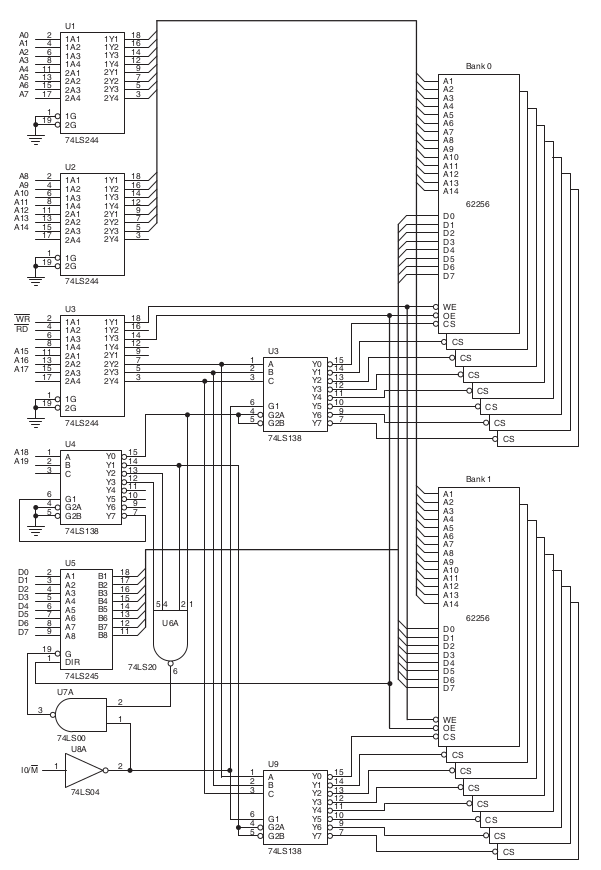
\includegraphics[width = 1\textwidth]{./figures/RAM.png}
  \caption{A 512K-byte static memory system using 16 62255 SRAMs.}
  \label{fig:ram}
\end{figure}
In the Figure \ref{fig:ram}, 16 \textit{62256}(32K x 8) static RAMs are interfaced to 8088 beginning at memory location 00000H to 7FFFFH(512K x 8). Here, two decoders select from 1 different RAM components and a third to select the other decodes for appropriate memory selection.
\begin{itemize}
  \item U4 selects the other two decoders. U3 selects sddresses beginning with 00 and U9 selects addresses beginning with 01. Extra pins of U4 remain for future extension.
  \item All address, data and control ($\overline{RD}$ and $\overline{WR}$) are buffered. Buffering is important when many devices appear in a single system. Excessive load without buffering can cause logic 0 output to rise above 0.V, maximum allowed in a system.
\end{itemize}
